\section{Numerical results}
\label{sec:numerical}

The theory says that the split-sample bound is valid at every sample size, but not how large the sample must be for
it to be useful. We measure this on simulated data whose total variation is known, and on two public data sets,
where the trimming at the certified level also gives a cohort.

\subsection{Simulations}
\label{sec:numharder}

Every design follows the contamination model \eqref{eq:contam}, with a common component of weight $1-a$ shared by $P$
and $Q$ and two design components $P_0$ and $Q_0$ of weight $a$, so that
$\TV(P,Q)=a\,\TV(P_0,Q_0)$ is known in closed form; $\alpha^\star=0.2$ unless a design says otherwise. The $\allNdesigns$ designs, listed in Table~\ref{tab:hardern80} and described in
Table~\ref{tab:harderdesigns} of the supplement, vary one feature at a time: where the contamination sits, the
dimension, how the signal is spread, its size, the type of data, and how smooth the difference of the densities is. In
the overlap and shift designs $P_0$ and $Q_0$ are $N(\pm\mu,I)$ on a $N(0,I)$ core, with $\mu$ along one
coordinate, along two or spread over all of them, so that $\{p>q\}$ is a half-space; the correlation flip changes the
sign of one correlation, the $t_3$ design the scale of one coordinate of a $t_3$ law, and the curves add or subtract a
bump to Brownian paths. The oscillating densities are those of Section~\ref{sec:upper}, which a fixed kernel sees less
and less as their frequency $\nu$ grows. One design is shaped on the RHC data of Section~\ref{sec:data}: it keeps the $\rrRhcNcovPaper$
covariates stored as numbers, takes a smoothed resample of the patients as the common component, and places $P_0$ and $Q_0$
in boxes at $\pm\rgSep$ pooled standard deviations in four coordinates.

Four methods certify a level of $\TV$. The split-sample bound $\widehat\alpha$ is Algorithm~\ref{alg:split} of the
supplement with the Laplace kernel, whose bandwidth is the median distance among the points each witness is fitted on.
The analytic baseline $\widehat\alpha_{\mathrm{an}}$ uses the threshold of Theorem~\ref{thm:plugin} and a Gaussian
kernel with its bandwidth fixed on a separate pilot draw of $1{,}000$ points from each law ($400$ and $2{,}000$ for
mixed types), not counted in $n$ or $m$. The other two run the same betting test on the labels of a
classifier, gradient boosting (GBM) or logistic regression \citep{pedregosa2011sklearn}, trained on the first half of
each sample as in \citet{naf2022hplb}. For reference we add two tests of $P=Q$, the permutation test of the MMD, with
the Gaussian kernel at the pilot bandwidth, and MMDAgg \citep{schrab2023aggregated}; they detect a difference but
certify nothing about its size. All methods see the same replicates, $\mnRepsPerSize$ per design and size, with $n=m$
doubling from $\harderNmin$ to $\harderNmax$ (mixed types: $n$ up to $400$, with $m=5n$). The four that certify are also
run at $\fourdigits{\harderNtwo}$ in the two designs of Table~\ref{tab:harderdesigns} that list it and, in every
design, at sizes doubling from $\fourdigits{\harderNtwo}$ to $\harderNcap$ until their power against $H_{0,0}$ reaches
$0.8$. The two tests of $P=Q$ are also run at $\fourdigits{\harderNtwo}$ on the narrow bump. The four that certify
test $H_{0,\alpha}$ at the levels $\alpha=j\alpha^\star/8$, $j=0,\dots,10$, with $\delta=0.05$.

We first check validity: a test may reject a true null, and the bound exceed $\alpha^\star$, with probability at most
$\delta$. At the level $\alpha=\alpha^\star$ the null $H_{0,\alpha^\star}$ holds, as $\TV(P,Q)$ is
exactly $\alpha^\star$: there, at $n=m=800$ (mixed types: $n=400$, $m=5n$), the betting test on the Laplace ramp
rejected $\mnBdTotal$ times in $\mnBdReps$ replicates in all, and at most $\mnBdMax$ in any one design. When $P=Q$, a
rejection of $H_{0,0}$ falsely claims a difference: on four designs in which both samples come from the same law,
over $\mnNullCells$ combinations of design and sample size, the same test rejected in $\mnNullPct\%$ of the replicates,
and at most $\mnNullMax$ in one combination. The analytic test never rejected in either case. For no method and no
combination does a binomial test at level $0.01$ find more rejections than $\delta$ allows, and in every design the
split-sample bound exceeded $\alpha^\star$ in at most a fraction $\mnAloGtMax$ of the replicates, well within the
$\delta$ that Corollary~\ref{cor:lower} allows (Section~\ref{app:experiments} of the supplement).

\begin{table}[t]
\centering
\footnotesize
\setlength{\tabcolsep}{5pt}
% Generated by scripts/aos_main_tables.py -- do not edit. Sample size n = m (mixed: n, m = 5n) for power 0.8 against H_{0,0} (first size with power >= 0.8, log-linear interpolation, two significant digits). Laplace ramp: results/aos/main (alpha = 0, Laplace kernel, all stored sizes and the alpha = 0 extension); analytic: tau = min{tau^P, tau^A} on the stored statistics; GBM, logistic: stored study; perm. MMD, MMDAgg: results/aos/baselines. Bold: smallest of the four tests that certify a level; italic: smaller of the two tests of P = Q.
\begin{tabular}{lccccccc}
\toprule
design & $\alpha^\star$ & $\widehat\alpha$ & $\widehat\alpha_{\mathrm{an}}$ & GBM & logistic & perm. & MMDAgg \\
 &  &  &  & + betting & + betting & MMD &  \\
\midrule
RHC-shaped, $d=33$ & $0.2$ & $\mathbf{{\le}100}$ & $450$ & $250$ & $230$ & $\mathit{{\le}100}$ & $\mathit{{\le}100}$ \\
overlap, $d=2$ & $0.1$ & $\mathbf{670}$ & $2{,}600$ & $5{,}100$ & $1{,}100$ & $\mathit{340}$ & $400$ \\
overlap, $d=2$ & $0.2$ & $\mathbf{160}$ & $620$ & $720$ & $280$ & $\mathit{{\le}100}$ & $\mathit{{\le}100}$ \\
overlap, $d=10$ & $0.1$ & $\mathbf{890}$ & $11{,}000$ & $4{,}900$ & $1{,}300$ & $\mathit{510}$ & $670$ \\
overlap, $d=10$ & $0.2$ & $\mathbf{180}$ & $1{,}500$ & $690$ & $320$ & $\mathit{{\le}100}$ & $130$ \\
dense shift, $d=20$ & $0.2$ & $\mathbf{210}$ & $2{,}800$ & $650$ & $360$ & $\mathit{120}$ & $150$ \\
dense shift, $d=50$ & $0.2$ & $\mathbf{300}$ & $5{,}800$ & $730$ & $500$ & $\mathit{160}$ & $190$ \\
dense shift, $d=100$ & $0.2$ & $\mathbf{380}$ & $11{,}000$ & $1{,}000$ & $690$ & $\mathit{210}$ & $240$ \\
sparse shift, $d=50$ & $0.2$ & $\mathbf{300}$ & $5{,}800$ & $660$ & $530$ & $\mathit{160}$ & $180$ \\
correlation flip, $d=50$ & $0.2$ & ${>}12{,}800$ & ${>}12{,}800$ & $\mathbf{5{,}200}$ & ${>}12{,}800$ & ${>}800$ & ${>}800$ \\
small contamination, $d=2$ & $0.05$ & $\mathbf{900}$ & $5{,}100$ & $5{,}500$ & $3{,}500$ & $600$ & $\mathit{500}$ \\
mixed types, $m=5n$ & $0.2$ & $\mathbf{140}$ & $660$ & $390$ & $170$ & $\mathit{{\le}100}$ & $\mathit{{\le}100}$ \\
$t_3$ tails, $d=5$ & $0.2$ & $\mathbf{320}$ & $2{,}800$ & $1{,}000$ & ${>}12{,}800$ & $\mathit{220}$ & $300$ \\
curves, wide bump & $0.2$ & $\mathbf{270}$ & $1{,}300$ & $690$ & $390$ & $\mathit{180}$ & $240$ \\
curves, narrow bump & $0.2$ & $1{,}200$ & $11{,}000$ & $1{,}100$ & $\mathbf{420}$ & $1{,}200$ & $\mathit{1{,}000}$ \\
oscillating, $\nu=1$ & $0.5$ & $\mathbf{{\le}100}$ & $\mathbf{{\le}100}$ & $\mathbf{{\le}100}$ & $\mathbf{{\le}100}$ & $\mathit{{\le}100}$ & $\mathit{{\le}100}$ \\
oscillating, $\nu=4$ & $0.5$ & $230$ & $2{,}600$ & $\mathbf{150}$ & $10{,}000$ & $580$ & $\mathit{{\le}100}$ \\
oscillating, $\nu=16$ & $0.5$ & $2{,}900$ & ${>}12{,}800$ & $\mathbf{290}$ & ${>}12{,}800$ & ${>}800$ & ${>}800$ \\
oscillating, $\nu=64$ & $0.5$ & ${>}12{,}800$ & ${>}12{,}800$ & $\mathbf{720}$ & ${>}12{,}800$ & ${>}800$ & ${>}800$ \\
\bottomrule
\end{tabular}

\caption{Sample size $n=m$ (mixed types: $n$, with $m=5n$) at which each method reaches power $0.8$ against
$H_{0,0}$ at $\delta=0.05$, from $\mnRepsPerSize$ replicates per size, interpolated between the two sizes that bracket
$0.8$ and rounded to two significant digits; ${\le}\mnNmin$, ${>}\mnNcap$: reached at the smallest size, not reached
at the largest. Bold: the smallest among the four tests that certify a level of $\TV$; italic: the smaller of the last
two, which test $P=Q$ only. $\widehat\alpha$: the betting test of Theorem~\ref{thm:betting} on the Laplace ramp;
$\widehat\alpha_{\mathrm{an}}$: the analytic test \eqref{eq:test} with the Gaussian kernel; GBM, logistic: the betting test on the labels of
gradient boosting and logistic regression trained once on half of the data, a handicap removed in Figure~\ref{fig:recovery}; perm.\ MMD: permutation test
with the Gaussian kernel at the pilot bandwidth of the analytic test and $\abPermB$ relabelings; MMDAgg: the test of
\citet{schrab2023aggregated}; the last two were run up to $n=800$ ($\fourdigits{\harderNtwo}$ on the narrow bump), so
${>}800$ means not reached there. The analytic and permutation tests take their bandwidth from a separate pilot draw,
not counted in $n$ (Section~\ref{sec:numharder}).}
\label{tab:hardern80}
\end{table}

The next question is how many observations each method needs to detect the contamination, that is, to reject
$H_{0,0}$ with power $0.8$ (Table~\ref{tab:hardern80}). Against classifiers trained once on half of the data, the
split-sample bound needs the fewest observations among the methods that certify a level of $\TV$ in
$\mnNeightyRampBest$ of the $\allNdesigns$ designs, alone in $\mnNeightyRampBestAlone$. Gradient boosting needs fewer
where the kernel at its bandwidth barely sees the difference, on the correlation flip, whose population MMD is about
zero, and on the oscillating densities with $\nu\ge4$, and both classifiers need fewer on the narrow bump. Refitted on
the batches of the ramp, the best of the classifiers, default or tuned, has more power at $n=m=800$ than the
split-sample bound in $\mnPowBestClfAboveLap$ designs and less in $\mnPowLapAboveBestClf$
(Section~\ref{sec:baselines} of the supplement). The analytic baseline needs $\mnAnaOverRampLo$ to $\mnAnaOverRampHi$ times
as many observations as the split-sample bound (median $\mnAnaOverRampMed$, over the designs where both sizes are
interpolated), the price of a threshold that holds for every pair in the null. It fires close to where the design rule
\eqref{eq:samplesize} predicts, at $\mnTauFireRatioLo$ to $\mnTauFireRatioHi$ times the size at which $\tau(0)$ meets
the population MMD.

Detecting a difference without certifying its size takes fewer observations. The permutation test of the MMD is the
fastest of all methods, or tied for fastest, in $\mnNeightyPermBest$ designs, and where both sizes are interpolated the
split-sample bound needs $\mnNeightyRampOverPermLo$ to $\mnNeightyRampOverPermHi$ times as many observations (median
$\mnNeightyRampOverPermMed$). The split-sample bound spends a quarter of each sample on fitting alone and pays for
betting, while the permutation test also takes its bandwidth from the pilot draw; the ratio falls below one only on the
oscillating density with $\nu=4$.

\begin{figure}[t]
\centering
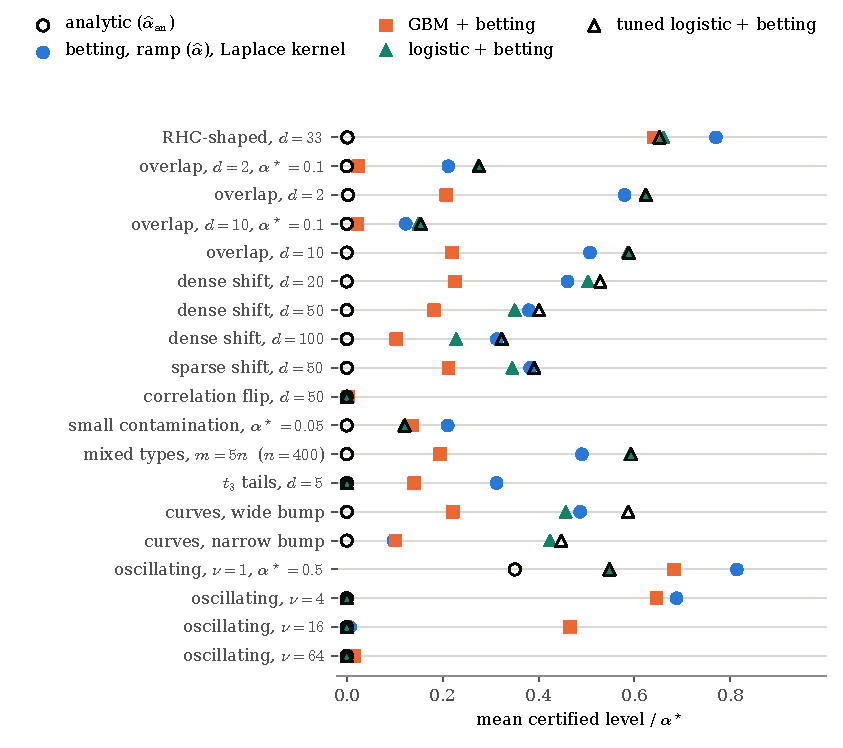
\includegraphics[width=\textwidth]{figs_aos/fig_recovery_main.pdf}
\caption{How much of $\alpha^\star$ each lower bound recovers at $n=m=800$ (mixed types: $n=400$, $m=5n$): the mean
over $\mnRecReps$ replicates of the largest level $j\alpha^\star/8$ it certifies divided by $\alpha^\star$, with $0$
when it certifies none, on a grid that uses the known $\alpha^\star$; $\alpha^\star=0.2$ unless shown, $\delta=0.05$;
classifiers: labels bet on the batches of the ramp.}
\label{fig:recovery}
\end{figure}

Detection certifies only the first level of the grid, and the bound is meant to certify as much of $\alpha^\star$ as
it can. We measure this by the recovery, the mean over replicates of the largest certified level divided by
$\alpha^\star$. The grid $j\alpha^\star/8$ uses the known $\alpha^\star$ only to express the levels as fractions of
it, and its largest level below $\alpha^\star$ is $7\alpha^\star/8$, so a valid bound recovers at most about
$\rcGridCeiling$. At $n=m=800$ the split-sample bound recovers a median $\mnRecRampMedian$ and a mean
$\mnRecRampMean$ over the designs, at most $\mnRecRampMax$, and $\mnRecRhcRamp$ on the RHC-shaped design
(Figure~\ref{fig:recovery}), while the
analytic baseline recovers a visible fraction only on the oscillating density with $\nu=1$, $\mnRecAnalyticMax$.

No bound recovers all of $\alpha^\star$ at this size. Near $\alpha^\star$ the excess of every function over $\alpha$ is
small, and a bet needs many pairs to detect a small excess: even the oracle that runs the same test on the better of
$\mathbf 1\{p>q\}$ and a level set of $p/q$ recovers a median $\rcOracleMedEightHundred$. Relative to this oracle,
with $\rcReps$ replicates per size below $800$, the recovery of the split-sample bound has median $\rcRatioMedHundred$, $\rcRatioMedTwoHundred$, $\rcRatioMedFourHundred$
and $\rcRatioMedEightHundred$ at $n=m=100$, $200$, $400$ and $800$, and the ratio is larger at $800$ than at $100$ in
$\rcRatioGrows$ of the $\rcRatioGrowsOf$ designs; in the other two the bound certifies almost nothing at any size
(Figure~\ref{fig:recoverycurves} of the supplement shows the curves).

Tuned classifiers can recover more than the split-sample bound where their model fits $\{p>q\}$. Refitted on the
batches of the ramp, unlike in Table~\ref{tab:hardern80}, so that all methods bet on the same observations, tuned
logistic regression recovers more than the bound in $\wtllosses{\mnWtlRecLogitTuned}$ designs and less in
$\wtlwins{\mnWtlRecLogitTuned}$, differences within two paired standard errors counting as ties, mostly more where
$\{p>q\}$ is a half-space, and tuned gradient boosting recovers more, at two decimals, on several designs, among them
the $t_3$ tails and the oscillating densities with $\nu\le16$; with default settings, the bound's mean recovery is
higher than that of the better of the two classifiers in $\mnRampAboveBestMatched$ of the $\allNdesigns$ designs and
lower in the others (Section~\ref{sec:baselines} of the supplement).
We keep the ramp as the default because it needs no tuning beyond the median-distance bandwidth, the rates of Section~\ref{sec:rates} are proved for it, and the program
that fits it also returns the trimming of Section~\ref{sec:trimming}. Validity does not depend on this choice: an
analyst who trusts a classifier on their data can bet on its labels instead (Section~\ref{sec:betting}).

In these designs the gain over an untrimmed witness comes mostly from where the witness is cut. The Gaussian witness
fitted once at $\alpha=0$, with no quadratic program, recovers a median $\abRecMedRampZero$ when cut at $\alpha=0$ and
$\abRecMedRampZeroCut$ when cut at the quantiles of the tested level, and the witness refitted at each level
$\abRecMedRamp$. At two paired standard errors refitting recovers more than the witness fitted at $\alpha=0$ and cut
at the tested level in $\wtlwins{\abWtlRecRampZeroCut}$ designs, as much in $\wtlties{\abWtlRecRampZeroCut}$ and less
in $\wtllosses{\abWtlRecRampZeroCut}$, and, at two decimals, that witness recovers more than the Laplace split-sample
bound in $\dvZeroCutAboveLap$ designs and less in $\dvZeroCutBelowLap$. Refitting gains on the $t_3$ tails, on both bumps and on
the oscillating density with $\nu=1$, and it is what consistency requires in general: a witness fitted at $\alpha=0$
can stop short of $\alpha^\star$ (Sections~\ref{sec:lower} and~\ref{sec:alphazero}).

The theory that favors the Laplace kernel holds on the line. Over the $\allNdesigns$ designs the Laplace kernel
recovers more than the Gaussian kernel in $\mnLapGaussWins$, $\mnLapGaussWinsLine$ of them oscillating densities on the
line, as much in $\mnLapGaussTies$, and less in $\mnLapGaussLosses$, where it is behind by at most
$\mnLapGaussLossMax$. In the $\mnMvDesigns$ multivariate designs, where our theory says nothing about the kernel, it is
slightly behind the Gaussian kernel: it needs fewer observations to detect in $\mnNeightyLapBelowGaussMv$ of them and
more in $\mnNeightyLapAboveGaussMv$, and recovers less in $\mnLapGaussLossesMv$ and more in $\mnLapGaussWinsMv$. Its
higher median recovery, $\mnRecRampMedian$ against $\mnRecGaussMedian$, comes from one design: on the oscillating
density with $\nu=4$ the recovery rises from $\mnRecNfourGauss$ to $\mnRecNfourLap$, which alone lifts the median.
Without it the medians are $\mnRecRampMedianNoNfour$ and $\mnRecGaussMedianNoNfour$, and the means over all designs
$\mnRecRampMean$ and $\mnRecGaussMean$. We keep the Laplace kernel as the default because its witness still sees
differences of high frequency that the Gaussian witness at the same bandwidth misses, as on this one-dimensional
density.

\subsection{Real data}
\label{sec:data}

We apply the split-sample bound and the analytic baseline to two public data sets, which give four contrasts. The
Right Heart Catheterization (RHC) study \citep{connors1996rhc} is an observational study of critically ill adults in
which the treatment is a catheter placed in the right side of the heart; of its $\rhcNtotal$ patients, $\cohNX$
received a catheter. We use its $\rrRhcNcovFull$ numeric and binary baseline covariates, the binary ones coded $0/1$,
standardized (Section~\ref{sec:rdbw} of the supplement lists them). The National Health and Nutrition Examination
Survey (NHANES) \citep{nhanes2012,john2019mims}, cycles 2011--2014 pooled, provides wrist accelerometry, from which we
take curves: for each participant, the mean over the valid days of $\log(1+\mathrm{MIMS})$ in each hour of the day,
with MIMS the monitor-independent movement summary, a curve on $24$ points. As an illustration on functional data, we
compare children aged 6--11 with older adults aged 60--79, younger adults aged 20--39 with the same older adults, and
body mass index below $25$ with $30$ or above within ages 20--59, which holds age roughly fixed; we call these the
child, the adult age and the body-mass contrasts. NHANES is a multistage survey, and we ignore its weights and design,
so these bounds concern the laws of the sampling process rather than the population of the United States. The
independence the betting test needs then holds only approximately, since participants share households and sampling
units; assigning whole sampling units to the batches gives the same or higher minima, though pairs within a batch can
still share a unit (Section~\ref{sec:rdbw}).

Every reported split-sample bound uses the Laplace kernel, with the median distance on batch $0$ as bandwidth for both
witnesses, a rule that, as in the simulations, uses only fitting data. The analytic baseline uses a Gaussian kernel with its
bandwidth fixed on a $30\%$ pilot sample of each group, and is computed on the other $70\%$ only. Each contrast is
reported at $\delta=0.05$, with no correction for the three NHANES contrasts.

\begin{table}[t]
\centering
\small
\setlength{\tabcolsep}{2.3pt}
% Generated by scripts/aos_main_tables.py -- do not edit. Analytic: scripts/exp_valid_bandwidth.py --threshold aos (tau = min{tau^P, tau^A}), pilot route; split-sample: Laplace kernel, genuine quantile cut points, eight splits (results/aos/main/raw/realdata_laplace). RHC: the 45 covariates (rhc_full; --rhc-covariates full).
\begin{tabular}{lrrcccccccc}
\toprule
 & & & \multicolumn{5}{c}{analytic ($\widehat\alpha_{\mathrm{an}}$), pilot bandwidth} & & \multicolumn{2}{c}{split-sample} \\
\cmidrule(lr){4-8}\cmidrule(lr){10-11}
contrast & $n$ & $m$ & $\widehat D_0$ & $\tau(0)$ & $n_{\mathrm{fire}}$ & $\alpha_{\mathrm{last}}$ & bisection & & $\widehat\alpha$ (min) & $\widehat\alpha$ (avg.\ e-value) \\
\midrule
RHC arms & 2{,}184 & 3{,}551 & 0.122 & 0.089 & 1{,}006 & 0.00 & 0 &  & 0.35 & 0.35 \\
ages 6--11 vs.\ 60--79 & 1{,}969 & 2{,}300 & 0.457 & 0.100 & 72 & 0.30 & 0.3375 &  & 0.75 & 0.80 \\
ages 20--39 vs.\ 60--79 & 2{,}519 & 2{,}300 & 0.209 & 0.094 & 342 & 0.05 & 0.0625 &  & 0.35 & 0.40 \\
BMI ${<}25$ vs.\ ${\ge}30$ & 1{,}627 & 2{,}008 & 0.075 & 0.109 & 2{,}633 & -- & -- &  & 0.05 & 0.05 \\
\bottomrule
\end{tabular}

\caption{The two bounds on the four contrasts (the last three from NHANES), $\delta=0.05$, grid mesh $0.05$; $n,m$:
group sizes, of which the analytic baseline uses $70\%$ after a $30\%$ pilot. Analytic baseline: $\widehat D_0$ and
$\tau(0)$, its statistic and threshold at $\alpha=0$; $n_{\mathrm{fire}}$, the balanced size of \eqref{eq:samplesize};
$\alpha_{\mathrm{last}}$, the largest rejected grid level, and bisection, the largest level rejected when bisecting to
width $0.0125$ (Section~\ref{sec:alpha}), both at most the infimum \eqref{eq:alphaest}; `--': none. Split-sample
bound, Laplace kernel: the smallest bound over eight random splits and the level certified by the average of their
final wealths, each $\delta$-level for this kernel. The three NHANES statements hold jointly with probability at least
$1-3\delta$.}
\label{tab:realdata}
\end{table}

One split of the observations into the batches of Section~\ref{sec:betting} makes the bound depend on the split, so we
compute it on eight random splits and summarize them in two ways. Their minimum is a $\delta$-level bound, as it
exceeds $\alpha^\star$ only if every split does. The average rests on e-values, nonnegative statistics whose mean under
the null is at most one, as is the wealth of a betting test at any fixed time: at each level the wealths of the eight
tests at their horizon are e-values for $H_{0,\alpha}$, so by Markov's inequality their average reaches $1/\delta$
with probability at most $\delta$, whatever the dependence between the splits \citep{vovk2021evalues}. Either summary
is valid if fixed in advance, while reporting the larger of the two is guaranteed only at level $2\delta$. We report
the minimum. The average, shown in Table~\ref{tab:realdata} for comparison, certifies as much, and more on the two age
contrasts.

The minima say that more than $\mnRdChildMin$ of the distribution of daily profiles of children, and likewise of older
adults, has no counterpart in the other group, more than $\mnRdAgeMin$ for younger against older adults, and more than
$\mnRdBmiMin$ for the body-mass groups (Table~\ref{tab:realdata}). On RHC every split certifies $\mnRdRhcMin$, so more
than $\mnRdRhcMin$ of the covariate distribution of each arm has no counterpart in the other. On RHC and on the child
and adult age contrasts, $\mnRdRhcNoBet$, $\mnRdChildNoBet$ and $\mnRdAgeNoBet$ of the eight splits stop at a level
where the fitted cut points satisfy $\widehat t_b\le\widehat u_b$ in both batches, so that there is no ramp to bet on
and the bound is limited by the fitted witness rather than by the number of pairs; the others stop at a failed bet.
The minima depend on the kernel on two of the contrasts: with the Gaussian kernel they are the same on the age
contrasts, but $\mnRdRhcFullGaussMin$ on RHC, with the same $\rrRhcNcovFull$ covariates, and $\mnRdBmiGaussMin$ on body
mass (Section~\ref{sec:kernelfallback}). The analytic baseline rejects a positive grid level only on the age contrasts, $\alpha^\star>\mnPvChildLast$ and
$\alpha^\star>\mnPvAgeLast$; on body mass $\widehat D_0=\mnPvBmiDzero$ lies below $\tau(0)=\mnPvBmiTauzero$, and the
design rule asks for $\mnPvBmiFire$ observations per group. Bet on the batches of the ramp, the labels of the
classifiers of Section~\ref{sec:numharder} certify $\rrClfFullGbmHardMin$ on RHC, as the ramp does, except tuned
logistic regression, $\rrClfFullLogitTunedHardMin$, and their predicted probabilities certify between
$\rrClfFullLogitTunedSoftMin$ and $\rrClfFullGbmSoftMin$ (minima over the eight splits; Section~\ref{sec:rdbw}).

\subsection{From the contamination level to a cohort}
\label{sec:appcohort}

At the level $\alpha^\star$ itself, trimming both arms would give the common core $R^\star$, with density proportional
to $\min(p,q)$ for the covariate densities $p,q$ of the two arms. With $e$ the propensity score, the probability $e(x)$ that a patient with covariates $x$ receives the catheter
\citep{rosenbaum1983central}, $\pi$ the fraction of
catheterized patients and $\rho$ the pooled density, $\min(p,q)=\rho\min\{e/\pi,(1-e)/(1-\pi)\}$, an overlap population
in the sense of \citet{li2018balancing}, and for arms of equal size that of the matching weights of
\citet{ligreene2013matching}. As $p/q$ increases with $e$, $\alpha^\star$ is also the total variation between the laws
of $e(X)$ in the two arms. Replacing $e$ by a logistic fit and $\rho$ by the pooled sample in
$\alpha^\star=1-\int\min(p,q)$ gives $\rrPropFullPlug$ (bootstrap interval $(\rrPropFullPlugLo,\rrPropFullPlugHi)$),
an estimate that rests on the propensity model and certifies nothing (Section~\ref{sec:rdbw}). Trimming near
$\alpha^\star$ targets the patients for whom both treatments are plausible, as propensity trimming does with a model
\citep{yang2018asymptotic}, while the rules of Section~\ref{sec:intro} aim at positivity.

At the level $\alpha=\lcCohAlpha$ of the lower bound on RHC we trim both arms with the Gaussian kernel at the pooled
median distance, which Corollary~\ref{cor:alphalo} allows for any valid and consistent level, here one from the Laplace bound. The program \eqref{eq:qp} has a unique minimizer, as
the Gram matrix of the patients is positive definite. It gives positive weight to $\lcPoolKeptX$ of the $\cohNX$ catheterized patients and
$\lcPoolKeptY$ of the $\cohNY$ others, and fractional weight only to the $\lcPoolFracX$ and $\lcPoolFracY$ on which the
witness equals its cut (Proposition~\ref{prop:bangbang}(ii)), which carry fractions $\lcPoolFracMassX$ and
$\lcPoolFracMassY$ of the trimmed samples (Section~\ref{sec:rdbw}). With the Laplace kernel, whose witness on the line
is flat on the set it trims (Proposition~\ref{prop:excess}(iii)), the program at the same level leaves $\lpPoolFracX$ and $\lpPoolFracY$ patients with fractional
weight.

The cohort is a $\lcCohAlpha$-trimming of each arm. Proposition~\ref{prop:alphahat} and Corollary~\ref{cor:alphalo}
describe such trimmings for a kernel fixed in advance, while here the bandwidth is the pooled median. The cohort leaves the
largest standardized difference of the $\rrRhcNcovFull$ covariates at $\lcTrimSMD$, below the usual threshold $0.1$.
A trimming balances only what it sees. In a separate run on the $\rrRhcNcovPaper$ covariates stored as numbers, the
Laplace trimming at the level $\rrCohPaperAlpha$ of the bound on them leaves $\rrCohPaperOmitSmdAbove$ of the other $\rrRhcNcovAdded$ above $0.1$, against
$\rrAddedSmdAbove$ before trimming. Matching and overlap weights balance more tightly but need a propensity model,
whose covariates the overlap weights balance exactly by construction (Table~\ref{tab:cohort}). The $30$-day mortality
difference, $\lcUnwRD$ in the raw arms, is $\lcTrimRD$ under the trimming, with interval $(\lcTrimRDlo,\lcTrimRDhi)$,
and up to $\lcRDmax$ under the other weightings, with overlapping intervals. These are illustrations, not causal
estimates: they would estimate effects only under no unmeasured confounding, and the intervals ignore the estimation of
the weights. As $\lcCohAlpha$ is a lower bound on $\alpha^\star$, the trimming approaches the common core only as the
level approaches $\alpha^\star$ (Corollary~\ref{cor:alphalo}), and the level should be reported with any effect
estimated on the cohort.
